\begin{lstlisting}[language=Python]
import numpy as np
import matplotlib.pyplot as plt
import matplotlib.image as mpimg
from sklearn.cluster import KMeans

def function_1(img, parameter):
    temp = np.reshape(img, (img.shape[0] * img.shape[1], 3))
    model = KMeans(n_clusters=parameter, random_state=0, n_init=1).fit(temp)
    output = model.cluster_centers_[model.labels_]
    output = np.reshape(output, (img.shape[0], img.shape[1], 3))
    return output

imagem = mpimg.imread("data/araras.png")
output = function_1(imagem, 3)
# Plotagem das figuras 1, 2 e 3
\end{lstlisting}

\begin{figure}[H]
    \centering
    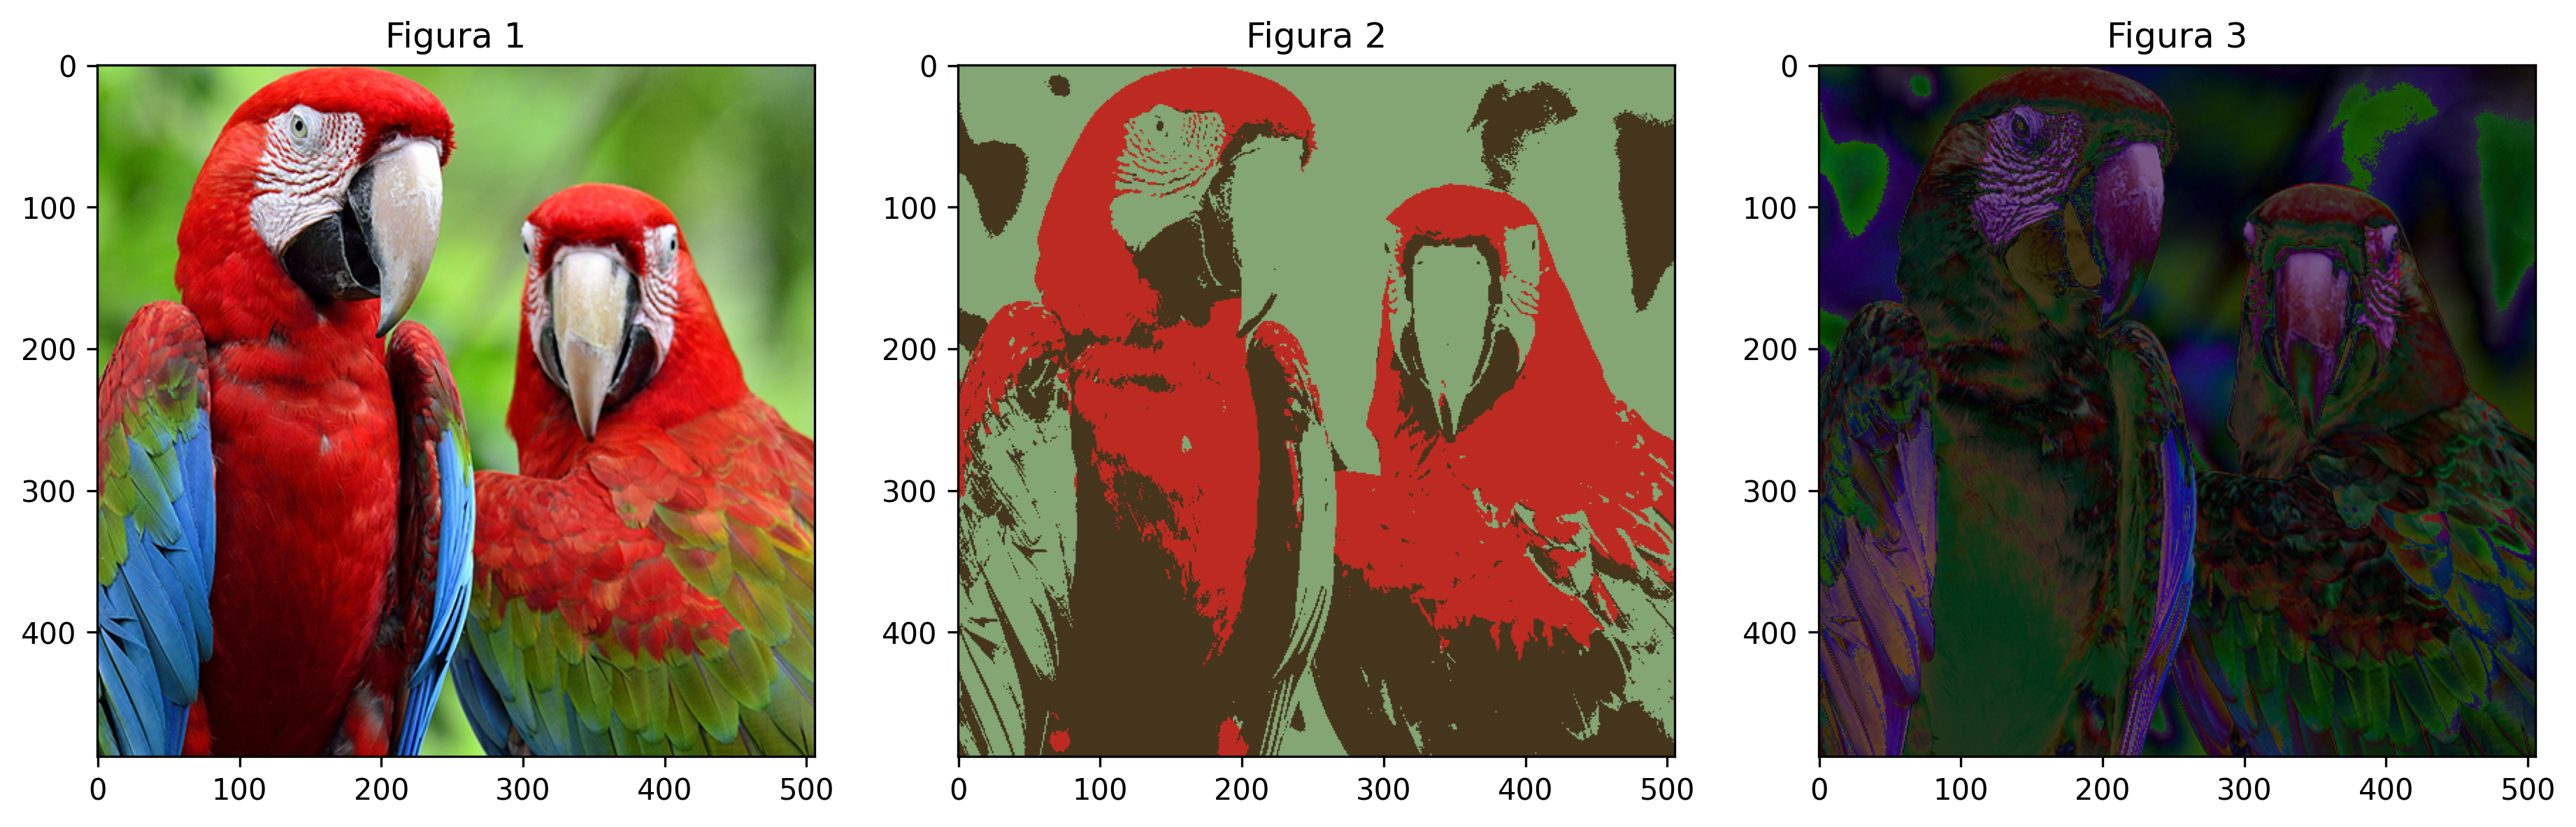
\includegraphics[width=0.9\textwidth]{../figures/5/initial_demo_k3.png}
    \caption{Demonstração inicial do algoritmo K-means com k=3}
    \label{fig:demo_k3}
\end{figure}

\newpage

\begin{lstlisting}[language=Python]
parameters = [3, 10, 30]
for parameter in parameters:
    output = function_1(imagem, parameter)
    # Plotagem das tres figuras para cada valor de parameter
\end{lstlisting}


\begin{figure}[H]
    \centering
    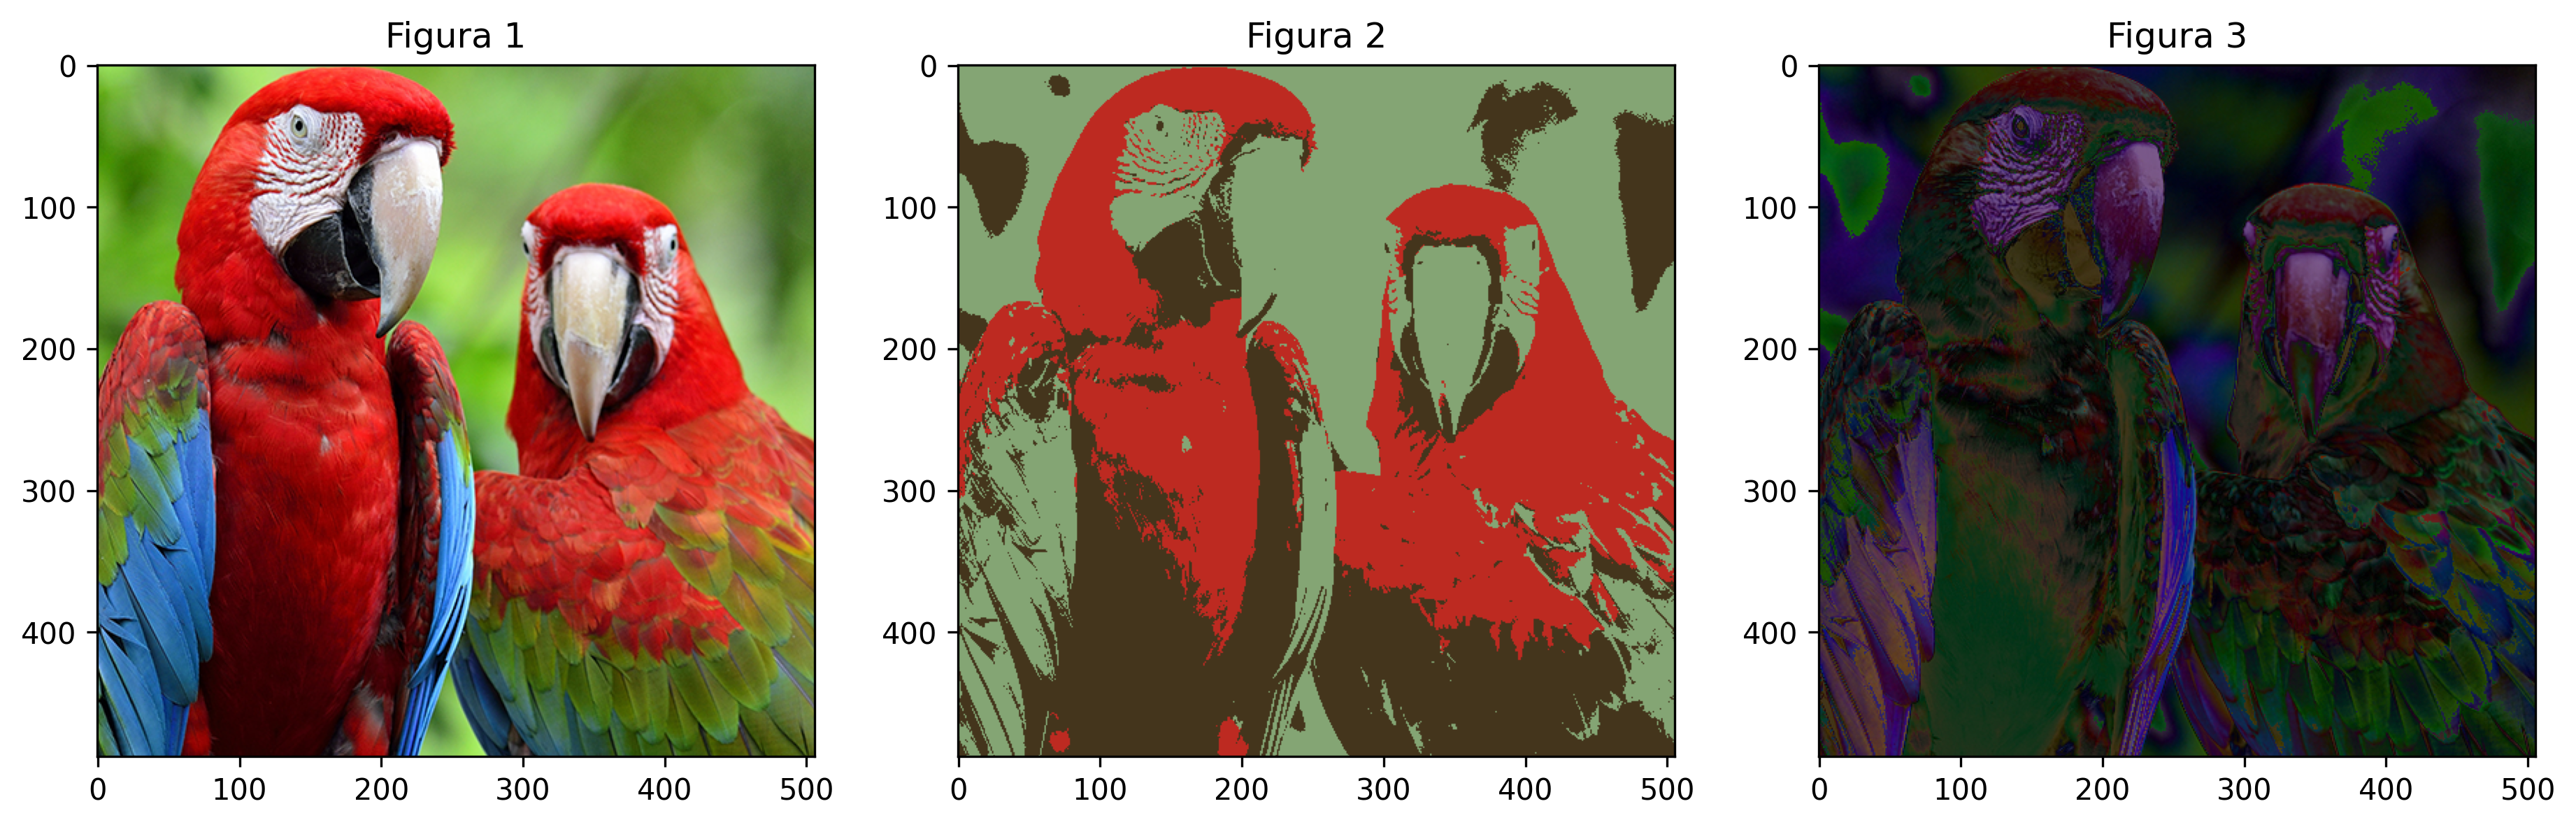
\includegraphics[width=0.9\textwidth]{../figures/5/parameter_3.png}
    \caption{Resultado com parameter = 3}
    \label{fig:param_3}
\end{figure}

\begin{figure}[H]
    \centering
    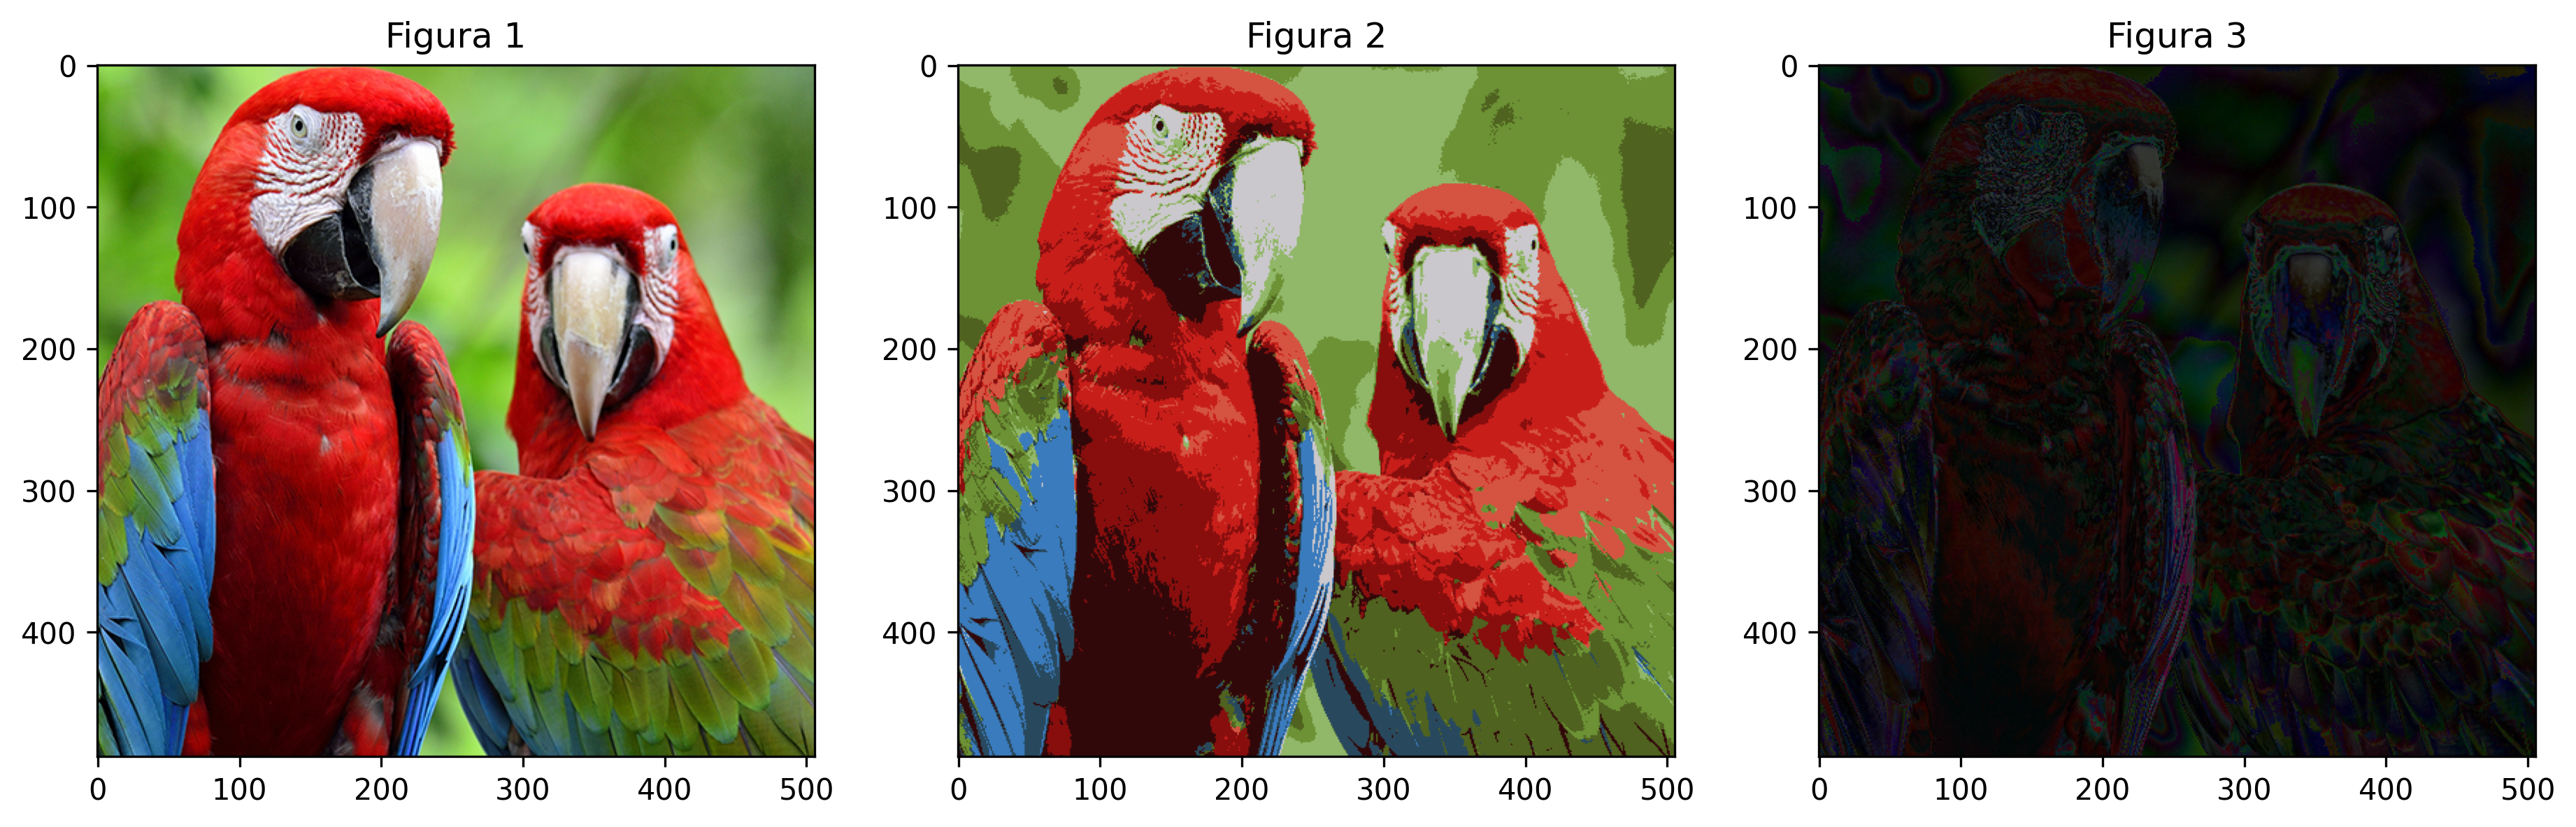
\includegraphics[width=0.9\textwidth]{../figures/5/parameter_10.png}
    \caption{Resultado com parameter = 10}
    \label{fig:param_10}
\end{figure}

\begin{figure}[H]
    \centering
    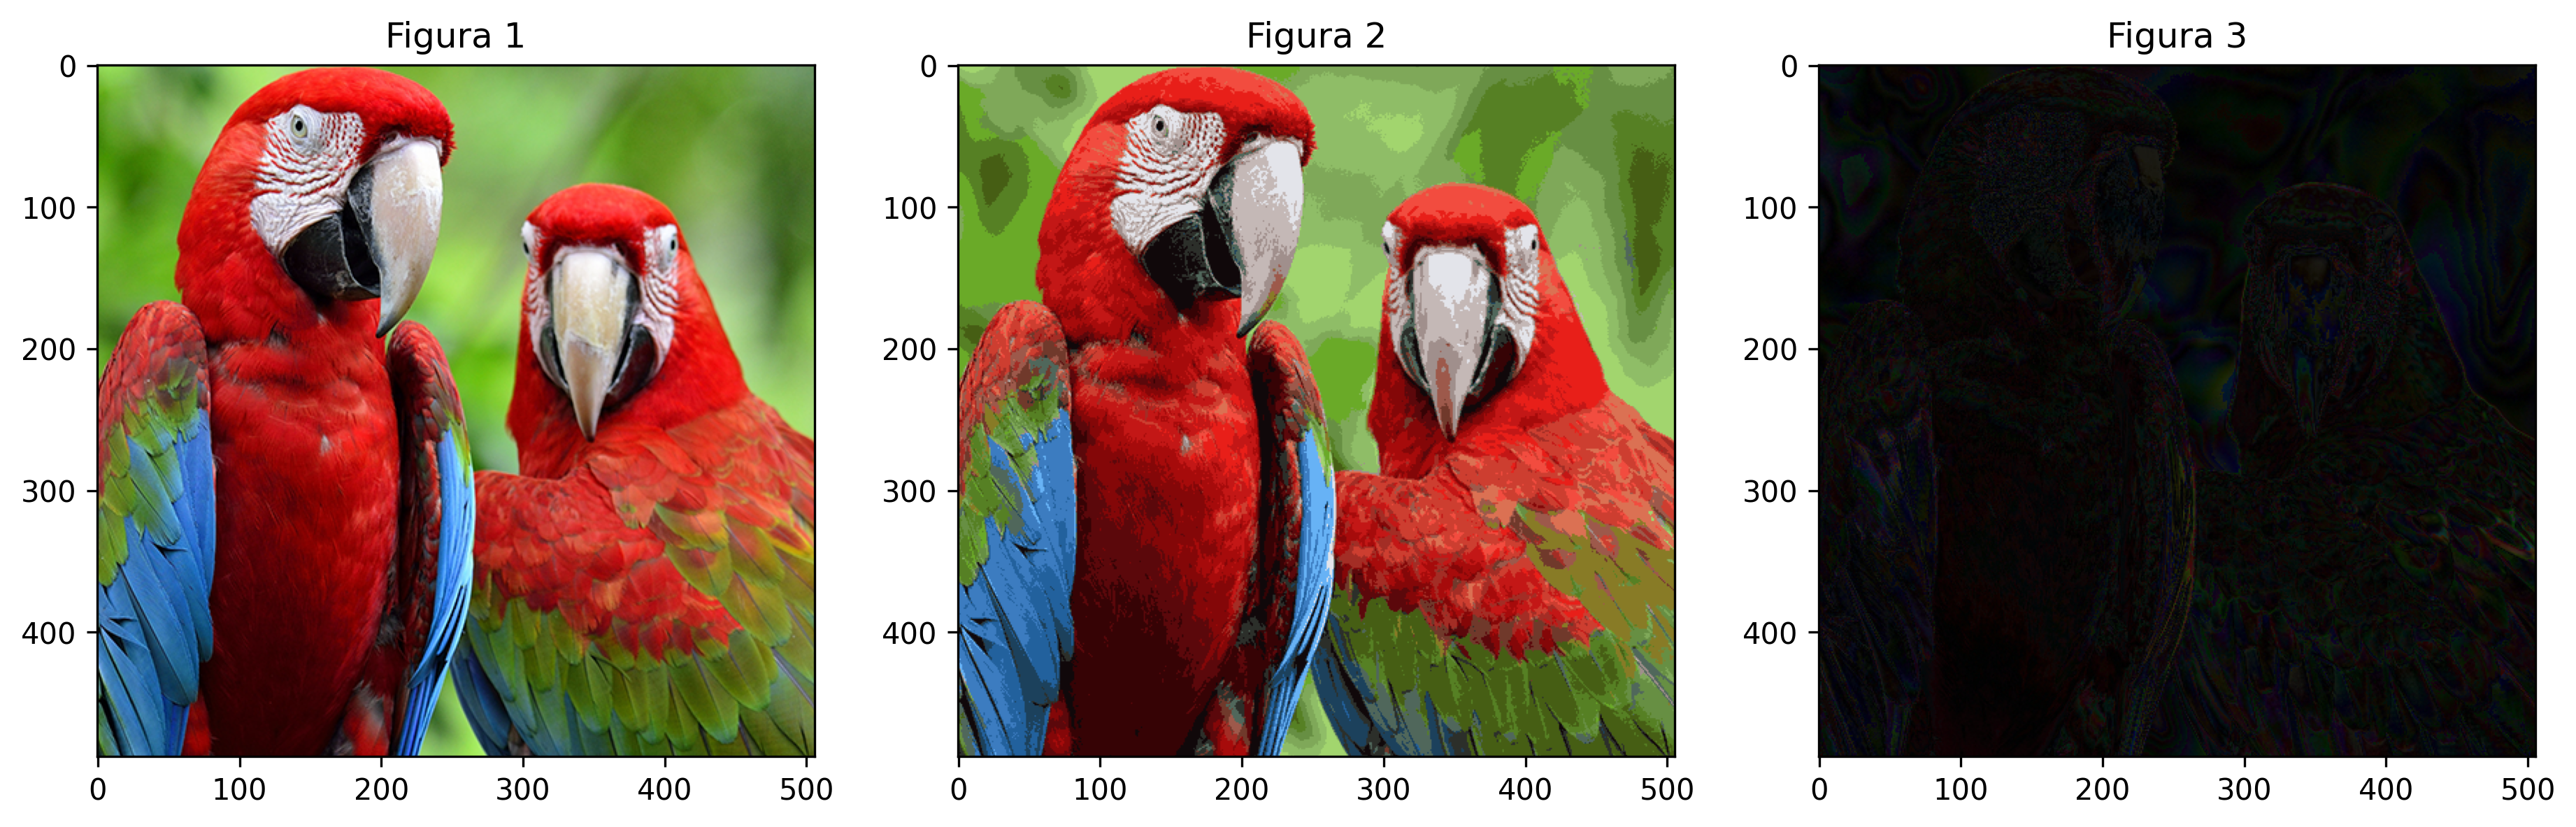
\includegraphics[width=0.9\textwidth]{../figures/5/parameter_30.png}
    \caption{Resultado com parameter = 30}
    \label{fig:param_30}
\end{figure}


A Figura 1 é a imagem original. A Figura 2 é a classificação de cada pixel em um dos três clusteres analisados. Cada cluster representa uma das três cores que melhor agrupavam as amostras em três grupos. A figura 3 é a parte da imagem que não foi incorporada na classificação anterior. Nela, foi retirado de cada pixel o cluster no qual ele foi classificado.

O \texttt{parameter} representa o número de clusteres que serão considerados na decomposição da imagem. Quanto maior o número de clusteres, mais cores serão consideradas na classificação, e a imagem resultante da Figura 2 se aproximará mais da imagem original. Já a Figura 3 se aproximará de uma imagem completamente preta, pois cada vez menos pixels serão classificados como parte do cluster errado.
